\subsection{\Large OpenGL and GLSL}
    \textbf{OpenGL}\cite{Sellers}\cite{Vries} is a cross-platform graphics API that is widely used for developing interactive 2D and 3D applications. It is a powerful and flexible tool that allows programmers to create rich visual experiences by drawing and manipulating 3D objects, textures, and lighting in a 3D environment. OpenGL is supported by a wide range of hardware and software platforms, including desktop and mobile devices, game consoles, and web browsers.

    \textbf{GLSL} (OpenGL Shading Language) is the programming language used to create shaders in OpenGL. Shaders are small programs that are executed on the graphics processing unit (GPU) and allow developers to write custom code to control the way that 3D objects are rendered. GLSL provides a wide range of built-in functions and data types that can be used to create a wide variety of effects, from simple per-pixel lighting to more advanced features such as depth of field, reflections, and more.
    
    In scientific applications, OpenGL and GLSL can be used to create interactive visualizations of complex data sets, such as simulations of physical phenomena, medical imaging, and more. The GPU's parallel processing capabilities allow for real-time interaction and manipulation of large data sets, which can be useful in fields such as data analysis, scientific research and discovery, and even interactive training simulations.
    
    One of the many advantages of using GLSL is the flexibility it provides in customizing and optimizing the pipeline of data, allowing the scientist to perform complex mathematical operation in the graphics pipeline, while being able to visualize the outcome in real time.
    
    In summary, OpenGL and GLSL are powerful tools that can be used in scientific applications to create interactive and visually rich visualizations of complex data sets. They allow scientists to analyze and manipulate data in real-time, making it a valuable addition to the scientific toolset.

    \textbf{Compute Shaders} are a specific type of shader that were introduced in OpenGL 4.3 and later. They are designed to perform general-purpose computation on the GPU, as opposed to the traditional rasterization-based pipeline used for rendering graphics. Compute shaders are executed on the GPU's stream processors, which are highly parallel units that can perform many calculations simultaneously.

    Compute shaders are written in GLSL and are executed on a three-dimensional grid of thread groups, each consisting of a fixed number of threads. The programmer defines the layout of the grid and the number of threads per group, and the GPU schedules the execution of the threads. The programmer can synchronize and communicate between different thread groups and between threads within the same group.

    % 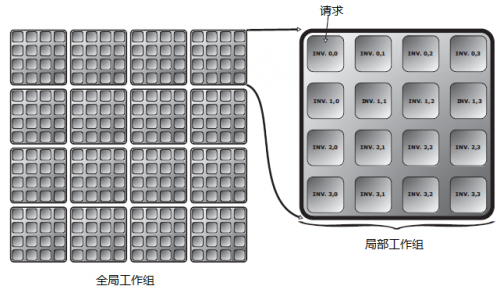
\includegraphics[width=3in]{resources/Compute.jpg}
    
    One of the advantages of using compute shaders is their ability to perform large amounts of data-parallel computation on the GPU. This can be much faster than performing the same computation on the CPU, especially for problems that can be easily parallelized. Additionally, compute shaders can also access memory resources such as textures and buffer objects, allowing the programmer to manipulate and store large data sets directly on the GPU.